\chapter{Matrix decomposition}


\section{Eigendecomposition}
\marginnote{Eigendecomposition}
Given a matrix $\matr{A} \in \mathbb{R}^{n \times n}$.
If the eigenvectors of $\matr{A}$ form a basis of $\mathbb{R}^n$,
then $\matr{A} \in \mathbb{R}^{n \times n}$ can be decomposed into:
\[ \matr{A} = \matr{P}\matr{D}\matr{P}^{-1} \]
where $\matr{P} \in \mathbb{R}^{n \times n}$ contains the eigenvectors of $\matr{A}$ as its columns and 
$\matr{D}$ is a diagonal matrix whose diagonal contains the eigenvalues of $\matr{A}$.



\section{Singular value decomposition}
\marginnote{Singular value decomposition}
Given a matrix $\matr{A} \in \mathbb{R}^{m \times n}$ of rank $r \in [0, \min\{m, n\}]$.
The singular value decomposition (SVD) of $\matr{A}$ is always possible and has form:
\[
    \matr{A} = \matr{U}\matr{\Sigma}\matr{V}^T
\]
where:
\begin{itemize}
    \item 
        $\matr{U} \in \mathbb{R}^{m \times m}$ is an orthogonal matrix with columns $\vec{u}_i$ called left-singular vectors.
    
    \item 
        $\matr{\Sigma} \in \mathbb{R}^{m \times n}$ is an orthogonal matrix with columns $\vec{v}_i$ called right-singular vectors.
    
    \item 
        $\matr{V} \in \mathbb{R}^{n \times n}$ is a matrix with $\matr{\Sigma}_{i,j} = 0$ (i.e. diagonal if it was a square matrix) and
        the singular values $\sigma_i, i = 1 \dots r$ on the diagonal.
        By convention $\sigma_1 \geq \sigma_2 \geq \dots \geq \sigma_r \geq 0$.
        Note that singular values $\sigma_j = 0$ for $(r + 1) \leq j \leq n$.
\end{itemize}

\marginnote{Singular value equation}
We can also represent SVD as a \textbf{singular value equation}, which resembles the eigenvalue equation:
\[  \matr{A}\vec{v}_i = \sigma_i\vec{u}_i \text{ for } i = 1, \dots, r \]
This is derived from:
\[ 
    \matr{A} = \matr{U}\matr{\Sigma}\matr{V}^T 
        \iff \matr{A}\matr{V} = \matr{U}\matr{\Sigma}\matr{V}^T\matr{V} 
        \iff \matr{A}\matr{V} = \matr{U}\matr{\Sigma}
\]

\subsection{Singular values and eigenvalues}
\marginnote{Eigendecomposition of $\matr{A}^T\matr{A}$ and $\matr{A}\matr{A}^T$}
Given $\matr{A} \in \mathbb{R}^{m \times n}$, we can obtain the eigenvalues and eigenvectors 
of $\matr{A}^T\matr{A}$ and $\matr{A}\matr{A}^T$ through SVD.

For $\matr{A}^T\matr{A}$, we can compute:
\[
\begin{split}
    \matr{A}^T\matr{A} & = (\matr{U}\matr{\Sigma}\matr{V}^T)^T(\matr{U}\matr{\Sigma}\matr{V}^T) \text{ using } (\matr{A}\matr{B})^T = \matr{B}^T\matr{A}^T \\
        & = (\matr{V}\matr{\Sigma}^T\matr{U}^T)(\matr{U}\matr{\Sigma}\matr{V}^T) \\
        & = \matr{V}\matr{\Sigma}^T\matr{\Sigma}\matr{V}^T \\
        & = \matr{V}\matr{\Sigma}^2\matr{V}^T
\end{split}    
\]
As $\matr{V}$ is orthogonal ($\matr{V}^T = \matr{V}^{-1}$), we can apply the eigendecomposition theorem:
\begin{itemize}
    \item The diagonal of $\matr{\Sigma}^2$ (i.e. the square of the singular values of $A$) are the eigenvalues of $\matr{A}^T\matr{A}$
    \item The columns of $\matr{V}$ (right-singular vectors) are the eigenvectors of $\matr{A}^T\matr{A}$
\end{itemize}

The same process holds for $\matr{A}\matr{A}^T$. In this case, the columns of $\matr{U}$ (left-singular vectors) are the eigenvectors.


\subsection{Singular values and 2-norm}
Given a symmetric matrix $\matr{A} \in \mathbb{R}^{n \times n}$, 
we have that $\matr{A}^T\matr{A} = \matr{A}^2 = \matr{A}\matr{A}^T$ (as $\matr{A}^T = \matr{A}$).

The eigenvalues of $\matr{A}^2$ are $\lambda_1^2, \dots,\lambda_n^2$, where $\lambda_i$ are eigenvalues of $\matr{A}$.
Alternatively, the eigenvalues of $\matr{A}^2$ are the squared singular values of $\matr{A}$: $\lambda_i^2 = \sigma_i^2$.
Moreover, the eigenvalues of $\matr{A}^{-1}$ are $\frac{1}{\lambda_1}, \dots, \frac{1}{\lambda_n}$.

\marginnote{2-norm using SVD}
We can compute the 2-norm as:
\[ \Vert \matr{A} \Vert_2 = \sqrt{\rho(\matr{A}^T\matr{A})} = \sqrt{\rho(\matr{A}^2)} = \sqrt{\max\{\sigma_1^2, \dots, \sigma_r^2\}} = \sigma_1 \]
\[ 
    \Vert \matr{A}^{-1} \Vert_2 = \sqrt{\rho((\matr{A}^{-1})^T(\matr{A}^{-1}))} = 
    \sqrt{\rho((\matr{A}\matr{A}^T)^{-1})} = \sqrt{\rho((\matr{A}^2)^{-1})} = \sqrt{\max\{\frac{1}{\sigma_1^2}, \dots, \frac{1}{\sigma_r^2}\}} = \frac{1}{\sigma_r}
\]
Furthermore, we can compute the condition number of $\matr{A}$ as:
\[ K(\matr{A}) = \Vert \matr{A} \Vert_2 \cdot \Vert \matr{A}^{-1} \Vert_2 = \sigma_1 \cdot \frac{1}{\sigma_r} \]



\subsection{Matrix approximation}
Given a matrix $\matr{A} \in \mathbb{R}^{m \times n}$ and its SVD decomposition $\matr{A} = \matr{U}\matr{\Sigma}\matr{V}^T$,
we can construct a rank-1 matrix (dyad) $\matr{A}_i \in \mathbb{R}^{m \times n}$ as: \marginnote{Dyad}
\[ \matr{A}_i = \vec{u}_i \vec{v}_i^T \]
where $\vec{u}_i \in \mathbb{R}^m$ is the $i$-th column of $\matr{U}$ and
$\vec{v}_i \in \mathbb{R}^n$ is the $i$-th column of $\matr{V}$.
Then, we can compose $\matr{A}$ as a sum of dyads:
\[ \matr{A}_i = \sum_{i=1}^{r} \sigma_i \vec{u}_i \vec{v}_i^T = \sum_{i=1}^{r} \sigma_i \matr{A}_i \]

\marginnote{Rank-$k$ approximation}
By considering only the first $k < r$ singular values, we can obtain a rank-$k$ approximation of $\matr{A}$:
\[ \hat{\matr{A}}(k) = \sum_{i=1}^{k} \sigma_i \vec{u}_i \vec{v}_i^T = \sum_{i=1}^{k} \sigma_i \matr{A}_i \]
Each dyad required $1 + m + n$ (respectively for $\sigma_i$, $\vec{u}_i$ and $\vec{v}_i$) numbers to be stored.
A rank-$k$ approximation requires to store $k(1 + m + n)$ numbers.

\begin{figure}[h]
    \centering
    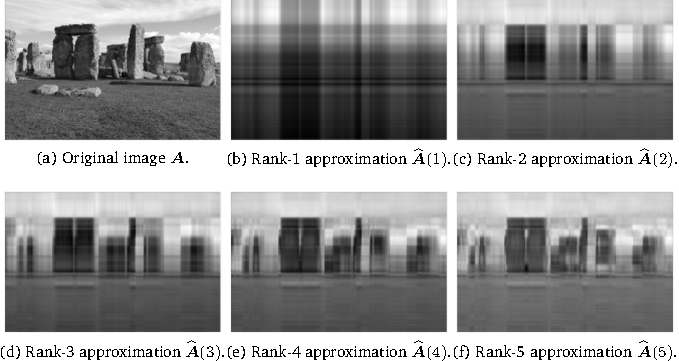
\includegraphics[width=0.60\textwidth]{img/_rank_k_approx.pdf}
    \caption{Approximation of an image}
\end{figure}



\section{Eigendecomposition vs SVD}
\begin{center}
    \begin{tabular}{m{16em} | m{16em}}
        \hline
        \multicolumn{1}{c|}{\textbf{Eigendecomposition}} & \multicolumn{1}{c}{\textbf{SVD}} \\
        \multicolumn{1}{c|}{$\matr{A} = \matr{P}\matr{D}\matr{P}^{-1}$} & \multicolumn{1}{c}{$\matr{A}=\matr{U}\matr{\Sigma}\matr{V}$} \\
        \hline
        Only defined for square matrices $\matr{A} \in \mathbb{R}^{n \times n}$ with eigenvectors that form a basis of $\mathbb{R}^n$ 
        & Always exists \\
        \hline
        $\matr{P}$ is not necessarily orthogonal & $\matr{U}$ and $\matr{V}$ are orthogonal \\
        \hline
        The elements on the diagonal of $\matr{D}$ may be in $\mathbb{C}$ 
        & The elements on the diagonal of $\matr{\Sigma}$ are all non-negative reals \\
        \hline
        \multicolumn{2}{c}{For symmetric matrices, eigendecomposition and SVD are the same} \\
        \hline
    \end{tabular}
\end{center}
